\section{Odds Ratio of Matching Paired Data}
\subsection{Set-up}
Let $X$ be the treatment variable.
\begin{itemize}
	\item $X = 1$: treatment group
	\item $X = 0$: control group
\end{itemize}

Let $Y$ be the outcome variable. $Y = 1$ or $Y = 0$.

In the $j$-th pair, let $(Y_{j,t}, Y_{j, mc})$ be the outcome status of the treated individual and the matched individual in the control group.

The event status can be one of the four possibilities $(0, 0), (0, 1), (1, 0), (1, 1)$.

\begin{figure}[H]
	\centering
	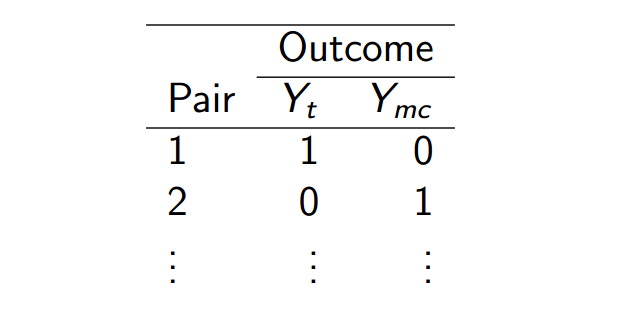
\includegraphics[width=0.5\linewidth]{fig/screenshot006}
	\caption{Paired Data List}
	\label{fig:screenshot006}
\end{figure}

The paired data can be represented into the contingency table.
\begin{figure}[H]
	\centering
	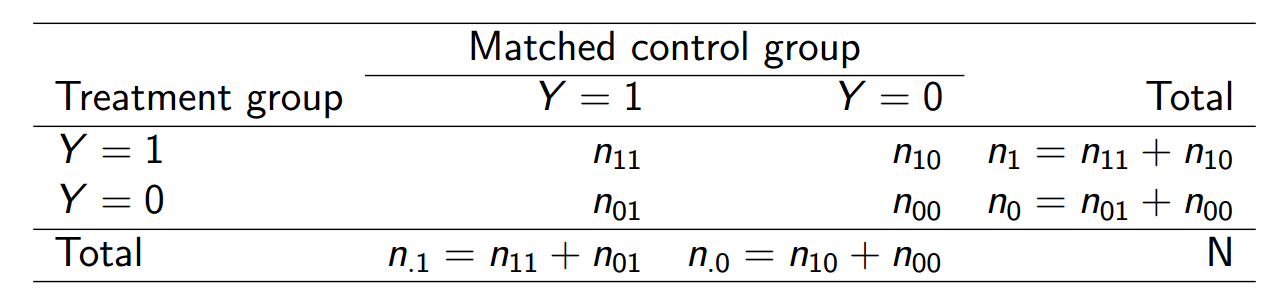
\includegraphics[width=0.7\linewidth]{fig/screenshot007}
	\caption{Contingency Table for Paired Data}
	\label{fig:screenshot007}
\end{figure}

Each frequency in the table represents number of pairs.
For instance, ``$n_{10}$'' means the number of pairs where the treated individuals have $Y= 1$ while the matched individual in the control group have $Y= 0$.

$N$ is the total number of pairs. $N = n_{11} + n_{10} + n_{01} + n_{00}$.

The proportion of $Y = 1$ 
\begin{itemize}
	\item in the treatment group is $(n_{11} + n_{10} / N)$.
	\item in the matched control group is $(n_{11} + n_{01} / N)$.
\end{itemize}

Hence, the difference of the proportions is $(n_{10} - n_{01}) / N$.

\subsection{Odds Ratio}
Use probabilities to represent paired groups.
\begin{figure}[H]
	\centering
	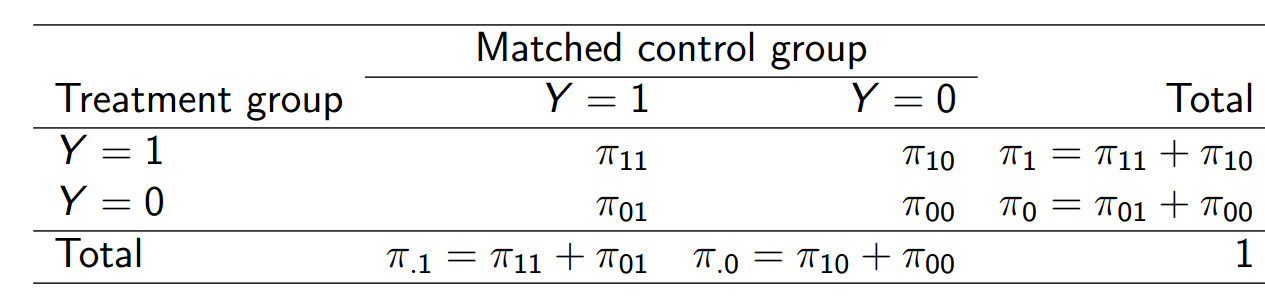
\includegraphics[width=0.7\linewidth]{fig/screenshot008}
	\caption{Probability in Contingency Table}
	\label{fig:screenshot008}
\end{figure}
In the table,
\begin{itemize}
	\item $\pi_{10} := \P(Y_{j,t} = 1, Y_{j, mc} = 0)$
	\item $\pi_{01} := \P(Y_{j,t} = 0, Y_{j, mc} = 1)$.
	\item $\pi_{1} := \P(Y_{j,t} = 1)$.
	\item $\pi_{.1} := \P(Y_{j, mc} = 1)$.
\end{itemize}

The odds ratio $\lambda = \pi_{10}/\pi_{01}$ measures the association between the outcome and the treatment.

An estimate of the odds ratio is $\hat{\lambda} = n_{10} / n_{01}$.

\subsection{Hypothesis Testing}
The null hypothesis is that the proportion of $Y = 1$ is the same in both treatment group and the matched control group.
\[H_0: \pi_{1} = \pi_{.1} \iff H_0: \pi_{10} = \pi_{01} \iff H_0: \lambda = 1\]

The alternative hypothesis is
\[H_1: \pi_1 \neq \pi_{.1}\]

The test statistic $T$ can be seen as approximately sampled from $\chi^2_1$ distribution for large sample.
\[T = \frac{(n_{10} - n_{01})^2}{n_{10} + n_{01}}\]

When consider continuity correction
\[T = \frac{(|n_{10} - n_{01}| - 1 )^2}{n_{10} + n_{01}}\]

Reject $H_0$ if $T > \chi_{\alpha,1}^2$.

\subsection{Example}
Johnson and Johnson (1972), in a study that was interested in
testing the theory that the tonsils protect the body against
invasion of the lymph nodes by a Hodgkin's disease virus,
obtained tonsillectomy data on 85 Hodgkin's cases and a sibling
of each case.

The data showed 41 tonsillectomies among the Hodgkin's cases
and 33 tonsillectomies among the siblings.
The pairing of a case with sibling means that the rates for the
two groups are not independent.

The pairing of a case with sibling means that the rates for the
two groups are not independent.
The pairing should be taken into account in the analysis in order
to achieve the best chance of detecting a departure from the null
hypothesis.
\[H_0: \text{Hodgkin's cases and their siblings have the same rates of
 tonsillectomy.}\]
The null hypothesis can be reduced to 
\[H_0: \text{The odds of tonsillectomy is the same.}\]

\begin{figure}[H]
	\centering
	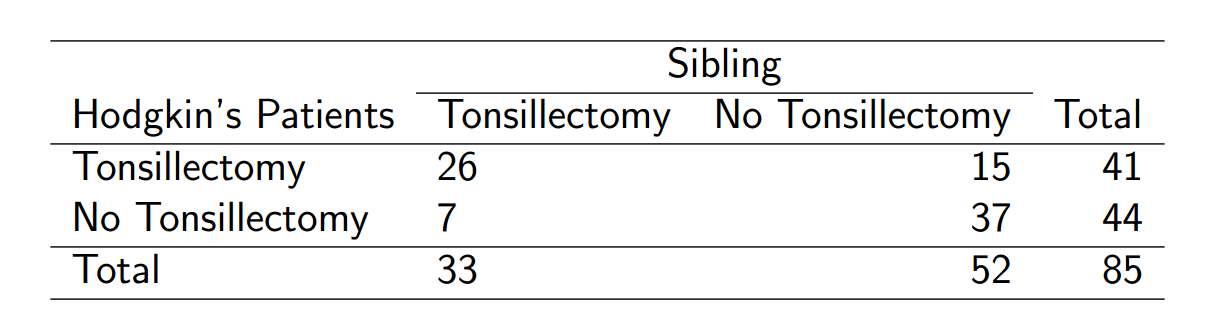
\includegraphics[width=0.7\linewidth]{fig/screenshot009}
	\caption{Contingency Table}
	\label{fig:screenshot009}
\end{figure}

\lstinputlisting[language=R]{code/l12-exp1.R}
